% !TEX root = ../main.tex
% !TEX program = XeLaTeX
% !TEX encoding = UTF-8 Unicode

\date{2018년 3월 21일}

\begin{frontmatter}
\title{레즈기어}
\author{김민규}
\address{서울대학교}
\begin{abstract}
Haspelmath, Martin. (1993). A Grammar of Lezgian. Berlin, Boston: De Gruyter Mouton, 110--121.
\end{abstract}
\end{frontmatter}

%%%%%
\section*{발제 범위 분배}
\begin{table}[h]
\begin{center}
\def\arraystretch{1.5}
\begin{tabular}{>{\sffamily}ccccl}
\hline
	&\itshape 발제자	&\itshape 발제 범위
	&\itshape 페이지	&\itshape 내용\\
\hline
1	&양재영	&Ch. 1--4	&pp. 1--51			&서론, 화자, 분절음운단위, 음소배열론\\
2	&김민규	&Ch. 5--7	&pp. 52--109			&(형태)음운적 교체, 강세, 명사 형태론\\
3	&김민규	&Ch. 8		&pp. 110--121		&형용사 형태론\\
	&		&Ch. 9		&pp. 122--162		&동사 굴절\\
4	&		&Ch. 10--12	&pp. 163--227		&동사 파생, 대명사, 부사 \& 후치사\\
5	&		&Ch. 14--15	&pp. 228--293		&수사 \& 불변화사, 명사구 \& 형용사구, 동사 결합가\\
6	&		&Ch. 16--19	&pp. 294--353		&절 통사론, 계사절, 등위접속, 관계절\\
7	&		&Ch. 20--21	&pp. 354--400		&보문절, 부사절\\
8	&		&Ch. 22--24	&pp. 401--441		&공지시, 의문문, 비교\\
\hline
\end{tabular}
\end{center}
\end{table}


\setcounter{section}{7}
\setcounter{subsection}{2}
\setcounter{subsubsection}{1}
\subsubsection{격들의 기능(계속)}

대부분의 처소격이 가지는 본래의 의미는 후치사의 사용으로 대치되었다. 그러나 처소격이 가지는 보다 추상적인 용례들이 존재한다.

\begin{table}[H]
\begin{center}
\begin{tabular}{llll}
\hline
격		&영문명		&본래의 의미	&현재의 사용, 추상적 의미\\
\hline
재상황격	&Adessive	&근처		&전동사 \textbf{Ag-}를 지닌 동사 등의 논항 (`by, to', 또는 `with')\\
재분리격	&Adelative	&근처로부터&보다 추상적 의미 (`로부터 빼앗다/원하다/배우다')\\
&&&\textbf{\^xun} `be, become'과 함께 사용하여 `가능'의 의미\\
&&&비자발적 행위자(Involuntary Agent)\\
재방향격	&Addirective	&근처로&도구, 태도(주로 추상 명사)\\

\hline
\end{tabular}
\end{center}
\end{table}

\pagebreak


\begin{table}[H]
\begin{center}
\begin{tabular}{llll}
\hline
격		&영문명		&본래의 의미	&현재의 사용, 추상적 의미\\

\hline
후상황격	&Postessive	&뒤에	&명사 \textbf{rak('ar)} `door', \textbf{pad} `side'와 함께: 보다 일반적 장소\\
&&&동사 \textbf{elqün} `turn', 명사 \textbf{pad} `side'와 함께: `toward'\\
&&&동사 \textbf{awa} `be, exist'와 함께: 소유자를 의미\\
&&&`in exchange for'; 몇몇 동사들과 후치사 \textbf{galaz} `with'의 논항\\
후분리격	&Postelative	&뒤로부터&명사 \textbf{rak('ar)} `door', \textbf{pad} `side'와 함께: 보다 일반적 장소\\
&&&감정(공포, 부끄러움)의 자극\\
후방향격	&Postdirective	&뒤로&`뒤'의 의미 없음, 오직 'toward'\\

\hline
하상황격	&Subessive	&아래에	&`지붕 아래', `그늘 아래', ...\\
&&&명사 \textbf{ajwan} `balcony' 등과 함께: 보다 일반적 장소\\
&&&동사 `mix', `participate' 등의 논항; 몇몇 전동사 동사의 논항\\
하분리격	&Subelative	&아래로부터&보다 추상적 의미 (`죽음이 너로부터 달아난다')\\
&&&동사 `hang'와 함께: 보다 일반적 장소;`free from' (`권리 없는')\\
&&&동사 `protect', `save'와 함께: `from, against' (`로부터 구하다')\\
&&&부분격 표현 (`--들 중에게서'); 감정의 자극\\
&&&주제 (`about'); 재료(material) (cf. \textbf{\^xun} `become' lit. `arise')\\
하방향격	&Subdirective	&아래로&(절대 처소격의 의미로 사용되지 않음)\\
&&&원인(`배고픔으로 죽다', `오지 않아서 화나다') 그러나 제한적\\

\hline
상상황격	&Superessive	&위에	&장소의 의미도 사용되며, 방향의 의미로도 사용\\
&&&몇몇 레즈기 마을 고유명사에 사용(그 외엔 내상황격 사용)\\
&&&감정(부러움, 만족, 기쁨, 자랑스러움)의 원인\\
&&&동사 \textbf{qʰürün} `laugh'의 대상\\
&&&상방황격을 대신하여 도구의 의미(최근 사용례 증가)\\
&&&동사 \textbf{hužumun} `attack' 등의 논항\\
상분리격	&Superelative	&위로부터&방향의 의미도 사용되며 경로(`across', `over')의 의미도 사용\\
&&&시간적 `in/after'의 의미 (`두 달 안에')\\
&&&시간적 `from, beginning with'의 의미 (`그 날 부터')\\
&&&비교문에 사용(24.1.1 참조); 여러 후치사의 논항\\
상방향격	&Superdirective	&위로&도구의 의미(`튀르크어로')\\
&&&추상 명사와 함께: 태도의 의미(`조심스럽게', `강한 목소리')\\
&&&무엇에 대해 성립하는지 표시; 시간적 `until'의 의미\\

\hline
내상황격	&Inessive	&위에	&장소의 의미도 사용되며, 방향의 의미로도 사용\\
&&&보다 추상적 의미(`학교에서', `마음에서')\\
&&&시간의 지속(`몇 년 동안', `세 시간 동안')\\
내분리격	&Inelative	&위로부터&기본적으로 방향의 의미로, `along, across'의 의미로도 사용\\
&&&감정의 원인; 보상(`in return for')\\
&&&후치사 \textbf{winiz} `up', \textbf{a\v{g}uz} `down'의 논항\\

\hline
\end{tabular}
\end{center}
\end{table}

\section{형용사 형태론}
\subsection{형용사의 굴절}
\begin{itemize}
\item 명사구 내에서 한정 용법으로 사용되는 형용사는 그 형태가 변화하지 않는다.
\item 비교급과 최상급 또한 형태론적으로 나타나지 않는다. (24.1 참조)
\item 따라서, 형용사 굴절에는 실질화(substantivization)과 형용사형 부사(adjectival adverbs) 밖에 존재하지 않는다.
\end{itemize}

\subsubsection{실질화}
\begin{itemize}
\item 실질화 접미사 \textbf{-di} (단수), \textbf{-bur} (복수)를 통해 명사구의 핵어가 될 수 있다.
\begin{figure}[H]
\centerline{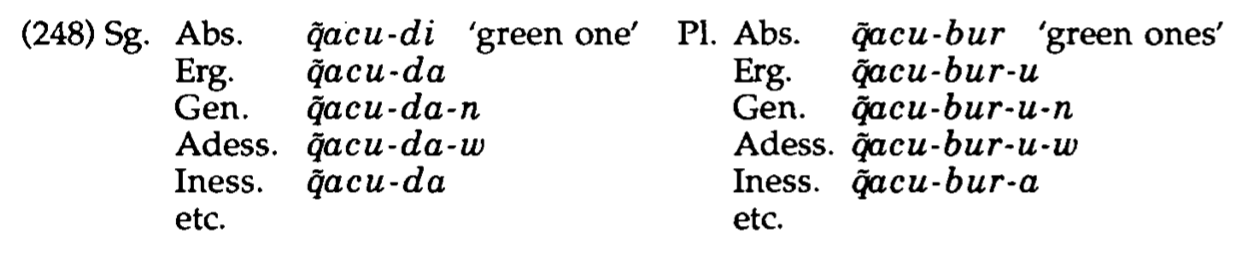
\includegraphics[width=.8\linewidth]{Lezgian/src/ex248.png}}
\end{figure}
\item 형용사 뿐만 아니라 다음과 같은 형태들도 실질화가 가능하다. 
\begin{itemize}
\item 분사 (19.1.2 참조)
\item 속격 명사구 (e.g. \textbf{Da\v{g}ustan.di-n} `다게스탄의' \textbf{Da\v{g}ustan.di-n-di} `다게스탄 사람')
\item 형용사 비교 소사 \textbf{\^xtin} `like', \textbf{q'wan} `as much as' 등 (24.2 참조) 및 여기서 비롯된 지시사와 의문사 \textbf{i\^xtin} `such', \textbf{iq'wan} `so much', \textbf{i\^xtin} `what kind?' 등 (11.3 참조)
\item \textbf{lahaj} 로 만든 서수(ordinal numerals) (13.1.3 참조)
\item 한정사 \textbf{mükü} `the other' (11.7.3 참조)
\end{itemize}
\item 한정사 \textbf{wiri} `all', \textbf{har} `every', \textbf{masa} `another' 또한 실질화와 비슷한 패러다임을 가지지만 절대격 단수만 불규칙적인 접미사를 가진다.
\begin{figure}[H]
\centerline{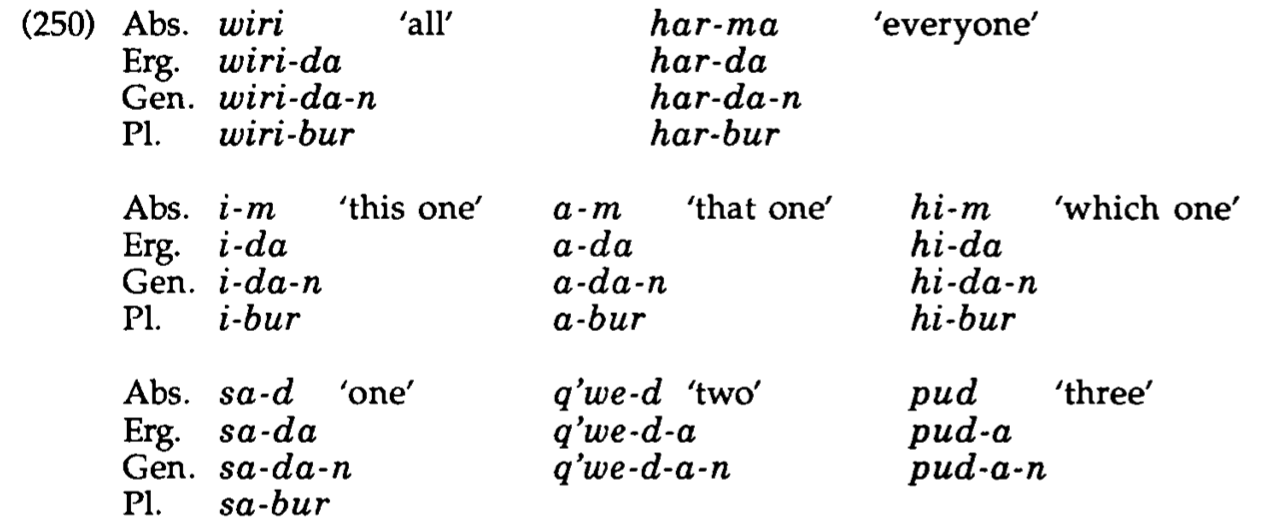
\includegraphics[width=.8\linewidth]{Lezgian/src/ex250.png}}
\end{figure}
\item 실질화된 형용사의 용법은 크게 3가지가 있다.
\begin{enumerate}
\item 대용어(anaphora)
\begin{figure}[H]
\centerline{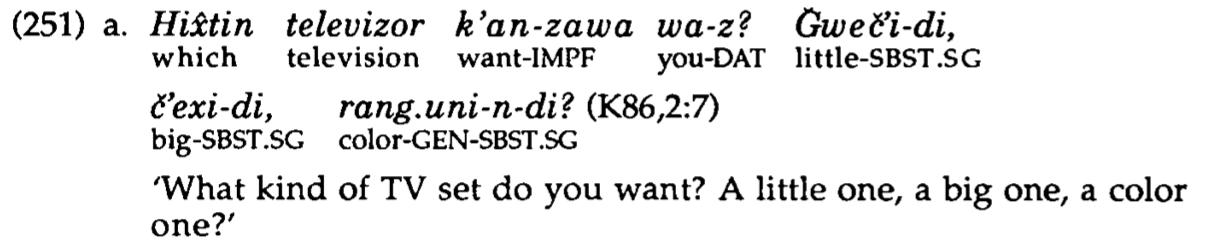
\includegraphics[width=.8\linewidth]{Lezgian/src/ex251a.png}}
\end{figure}
\item 형용사에서 명사로의 전환
\begin{figure}[H]
\centerline{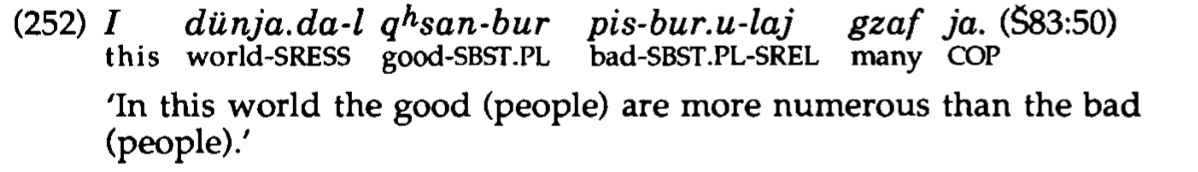
\includegraphics[width=.8\linewidth]{Lezgian/src/ex252.png}}
\end{figure}
\item 서술 용법의 형용사 (일반 형용사의 쓰임과 의미 차이가 별로 없다.)
\begin{figure}[H]
\centerline{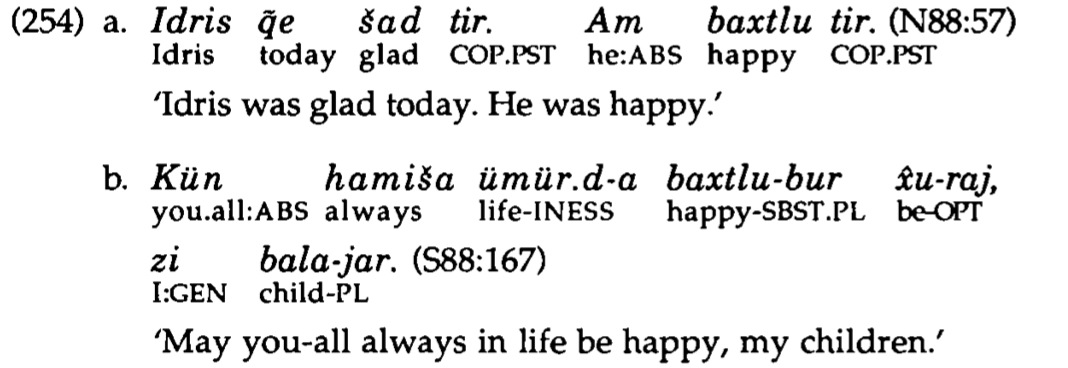
\includegraphics[width=.8\linewidth]{Lezgian/src/ex254.png}}
\end{figure}
\begin{itemize}
\item 서술 용법으로 사용할 경우 주어와 수 일치를 한다. (레즈기어의 유일한 일치 현상)
\end{itemize}
\end{enumerate}
\end{itemize}

\subsubsection{형용사형 부사}
\begin{itemize}
\item 레즈기어에는 부사를 만드는 접미사가 크게 두 개 \textbf{-dakaz} 와 \textbf{-diz/-z} 가 있고 몇몇 접미사가 더 있다.
\item \textbf{-dakaz} 와  \textbf{-diz/-z} 는 의미의 차이는 없지만, 후자가 더 빈번하다. 
\item \textbf{-dakaz}는 Axceh 방언에서 온 것으로 알려져 있고(Gadžiev 1954), 시 등에서 가끔 사용되며 산문에는 거의 나타나지 않는다. 러시아어 차용어 등에 부착 가능하다.
\item \textbf{-diz} 는 자음으로 끝나는 형용사, \textbf{-z} 는 모음으로 끝나는 형용사 뒤에서 사용되며, \textbf{n} 으로 끝나는 형용사는 두 접미사를 모두 취한다. (\textbf{n} 이 탈락하고 선행 모음을 비모음화하는 경우가 있다.)
\begin{figure}[H]
\centerline{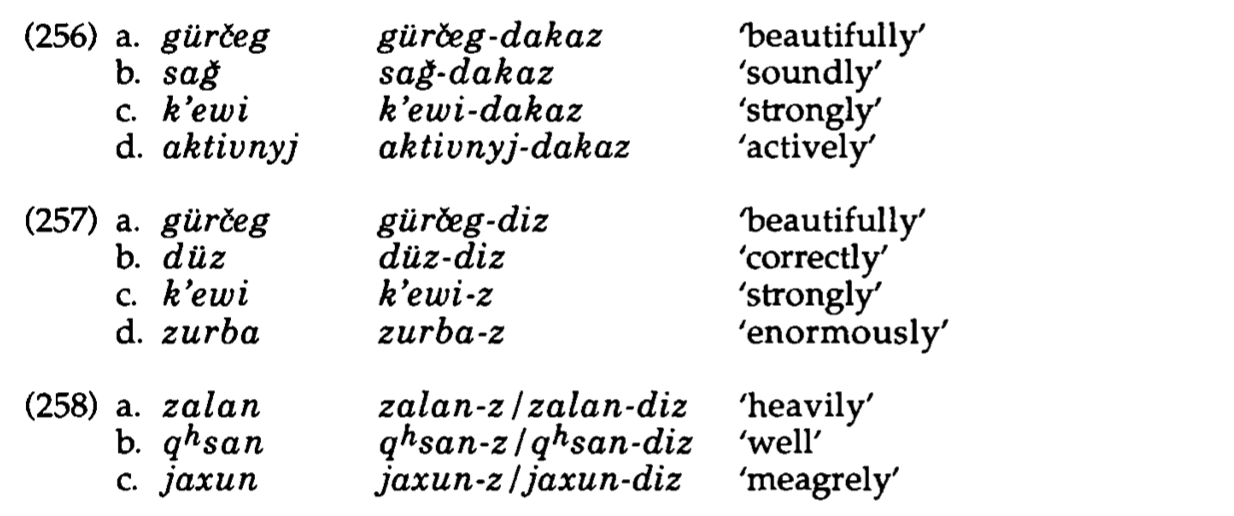
\includegraphics[width=.8\linewidth]{Lezgian/src/ex8-1-2-1.png}}
\end{figure}
\item 형용사형 부사의 가장 큰 기능은 동작의 방식/태도(manner)를 나타내는 것이다.
\begin{figure}[H]
\centerline{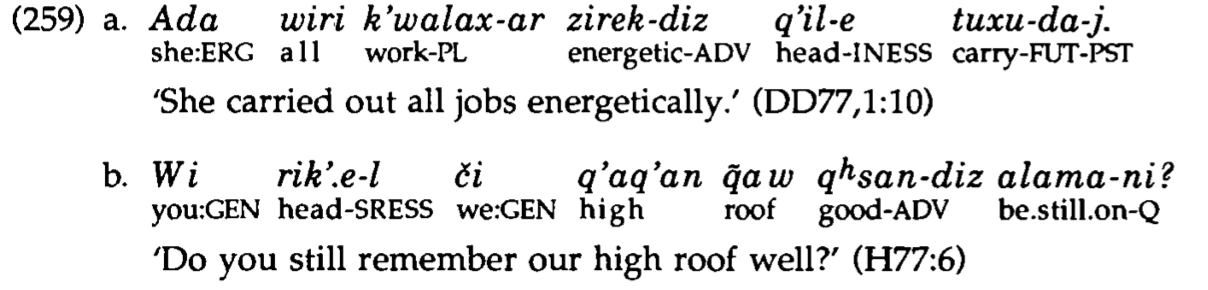
\includegraphics[width=.8\linewidth]{Lezgian/src/ex259.png}}
\end{figure}
\item 형용사형 부사는 공동-서술적 용법(copredicative)으로 사용될 수도 있다. 즉, 주어를 수식한다.
\begin{figure}[H]
\centerline{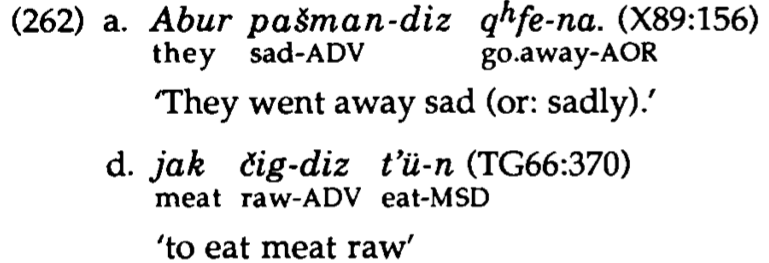
\includegraphics[width=.5\linewidth]{Lezgian/src/ex262.png}}
\end{figure}
\item 형용사형 부사는 미완료 부동사(imperfective converb) \textbf{-z} 와 형태론적으로만 일치하는 것이 아니라 그 쓰임에서도 유사성이 있다.
\begin{itemize}
\item 동사 \textbf{akun} `see'의 보어로 사용된다
\begin{figure}[H]
\centerline{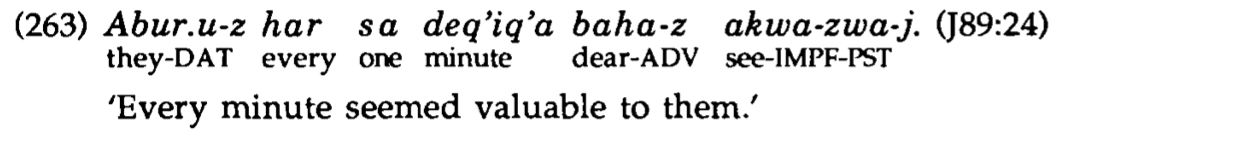
\includegraphics[width=.8\linewidth]{Lezgian/src/ex263.png}}
\end{figure}
\item 장소 계사 \textbf{ama} `be still' 와 함께 쓰인다.
\item 중첩이 가능하다.
\begin{figure}[H]
\centerline{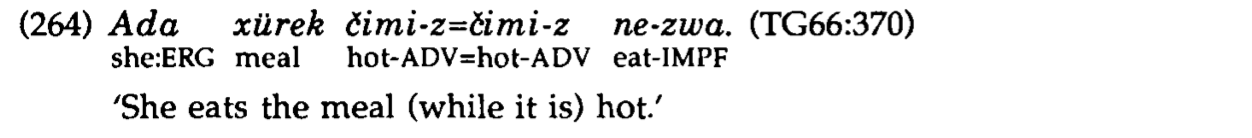
\includegraphics[width=.8\linewidth]{Lezgian/src/ex264.png}}
\end{figure}
\end{itemize}
\item 그 외에도 \textbf{-k'a}, \textbf{-Aba}, \textbf{-Aldi} 가 부착되기도 한다. (자세한 사항은 생략)
\item \textbf{-wileldi} (추상 접미사  \textbf{-wal}의 상방향격(superdirective) 형태) 또한 부사 접미사로서 매우 생산적이고 자주 사용된다. \textbf{-dakaz} 와 의미의 차이는 없다.
\begin{figure}[H]
\centerline{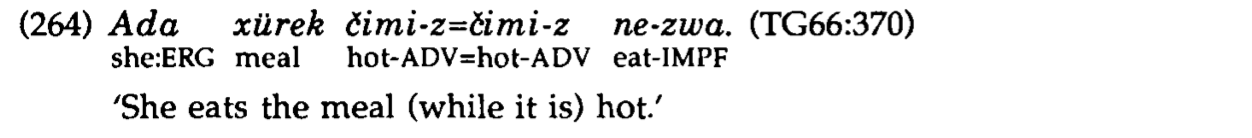
\includegraphics[width=.8\linewidth]{Lezgian/src/ex264.png}}
\end{figure}
\item 형용사가 별다른 접미사 없이 동사를 수식하여 부사처럼 사용될 수도 있다.
\end{itemize}

\subsubsection{형용사에 부착되는 서술 접미사}
\begin{itemize}
\item 서술 접미사 \textbf{-da} (과거형 \textbf{-daj}) 가 부착하여 서술적 기능을 할 수 있다고 레즈기어 문법서들이 서술하고 있다. (Uslar 1896, Gadžiev 1954, Ramaldanov 1980)
\begin{figure}[H]
\centerline{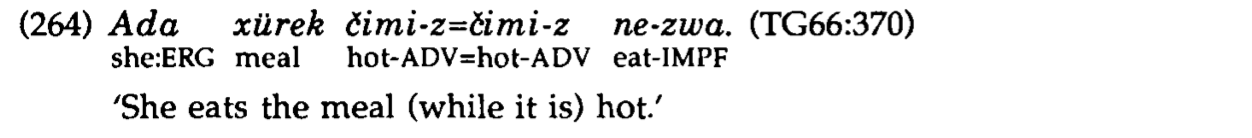
\includegraphics[width=.8\linewidth]{Lezgian/src/ex264.png}}
\end{figure}
\item 그러나 이 접미사는 현대 표준어에서는 사용되지 않는다.
\item 예외로, \textbf{k'anda} `wants', \textbf{čida} `knows',  \textbf{t'ada} `hurts',  \textbf{kič'eda} `fears' (9.5.2 참조) 등이 있으나, 본 문법서에서는 이들을 동사로 취급한다.
\item 미래 시제 접미사 \textbf{-da}가 이것과 분명히 관련이 있을 것이다. 
\begin{itemize}
\item 가장 가능성 있는 시나리오는 \textbf{-da}가 원래는 계사였고, 표준 계사 \textbf{-ja}와 장소 계사 \textbf{awa}가 어원적으로 연관이 있었을 것이다. \textbf{d/j}는 원래 성 표지였고 \textbf{aw-}는 전동사(preverb)였다. 이들이 형용사에 부착되어 (271)과 같은 형태로 사용되고, 동사의 특정 분사형에 부착되어 일반적인 현재 시제를 나타내었다가 나중에 습관적 또는 미래 상황을 나타내는 용법으로 변화했을 것이다. 그리고 형용사형은 더 이상 사용되지 않게 되고 \textbf{k'anda}와 같은 몇몇 형태에만 남게 되었고 이것이 동사가 되었을 것이다.
\end{itemize}
\item  \textbf{-da} 를 사용한다고 보고된 대부분의 문장은 (전부는 아니지만) 환경이나 심리 상태를 나타내는 문장들이다. (많아봐야 절대격 논항 하나를 취한다.)
\begin{figure}[H]
\centerline{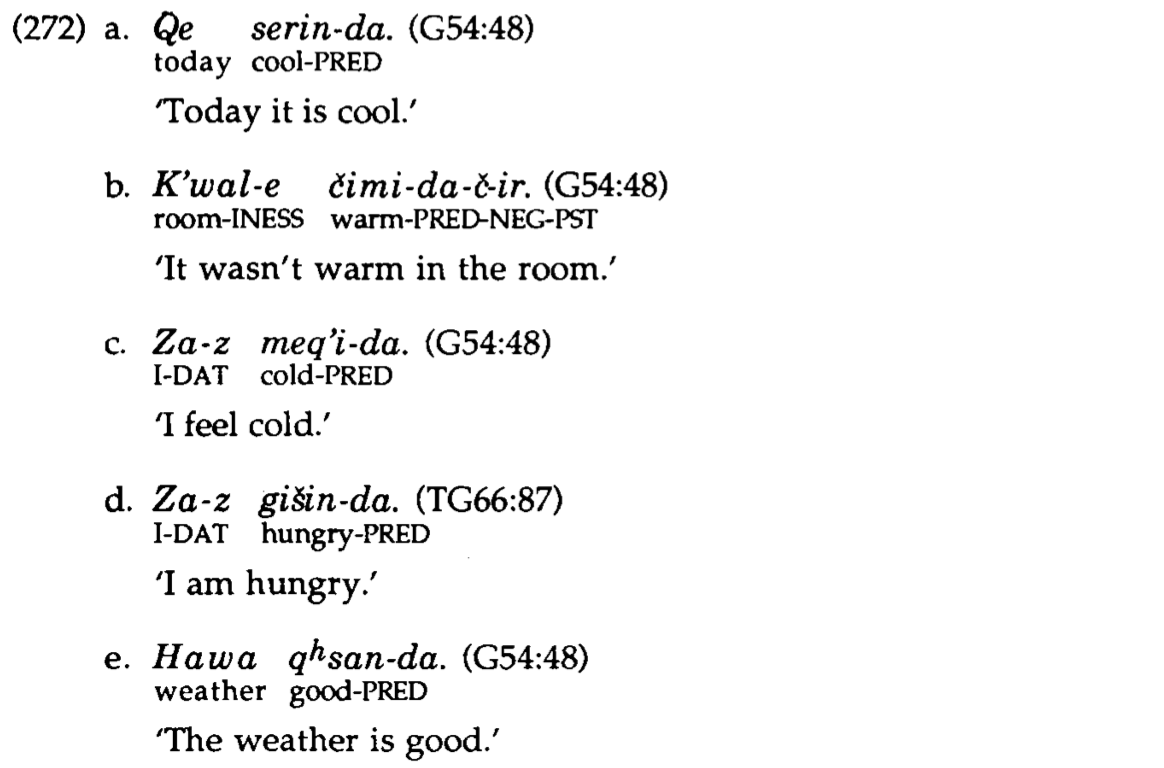
\includegraphics[width=.8\linewidth]{Lezgian/src/ex272.png}}
\end{figure}

\item 미완료 접미사 \textbf{-z(a)wa/-z(a)ma} 가 존재한다. 동사의 미완료 형이 미완료 부동사 형태(\textbf{-z})에 장소 계사 \textbf{awa} 가 결합 및 축약되어 \textbf{-z(a)wa}가 되는 것과 같은 원리이다.
\begin{figure}[H]
\centerline{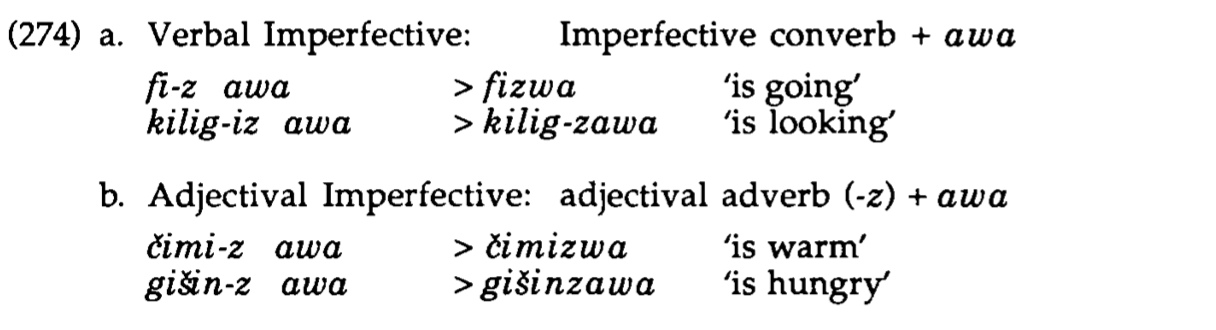
\includegraphics[width=.8\linewidth]{Lezgian/src/ex274.png}}
\end{figure}
\item 마찬가지로 환경 또는 심리 상태를 기술하는 형용사에 자주 사용된다.
\begin{figure}[H]
\centerline{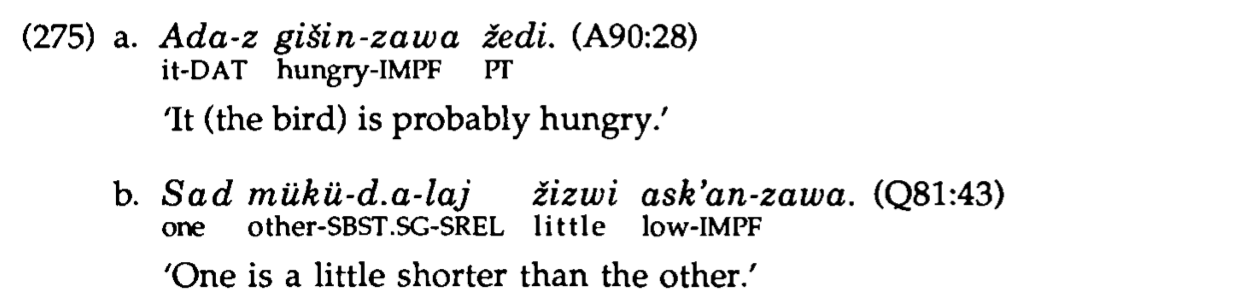
\includegraphics[width=.8\linewidth]{Lezgian/src/ex275.png}}
\end{figure}
\begin{figure}[H]
\centerline{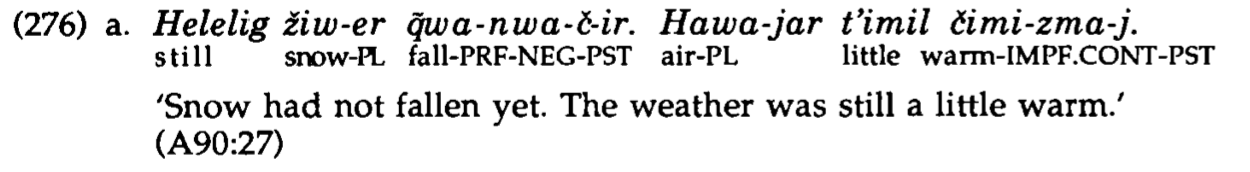
\includegraphics[width=.8\linewidth]{Lezgian/src/ex276a.png}}
\end{figure}
\item 형용사형 미완료 형태에 한 번 더 미완료 부동사가 부착될 수도 있다.
\begin{figure}[H]
\centerline{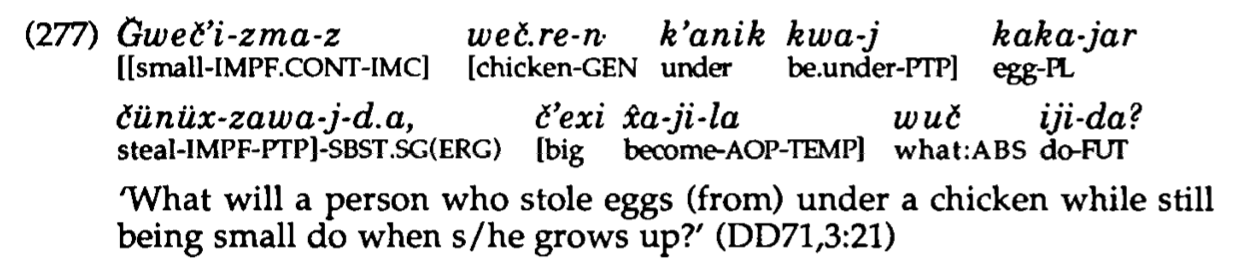
\includegraphics[width=.8\linewidth]{Lezgian/src/ex277.png}}
\end{figure}
\end{itemize}

\subsubsection{국적 형용사}
\begin{itemize}
\item 국적을 나타내는 단어는 명사로도, 형용사로도 사용된다.
\begin{figure}[H]
\centerline{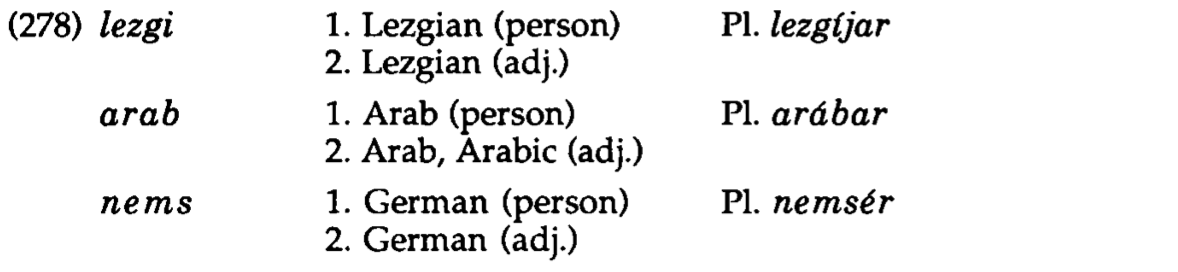
\includegraphics[width=.8\linewidth]{Lezgian/src/ex278.png}}
\end{figure}
\item 속격 복수 형태는 형용사 용법으로만 사용된다.
\begin{figure}[H]
\centerline{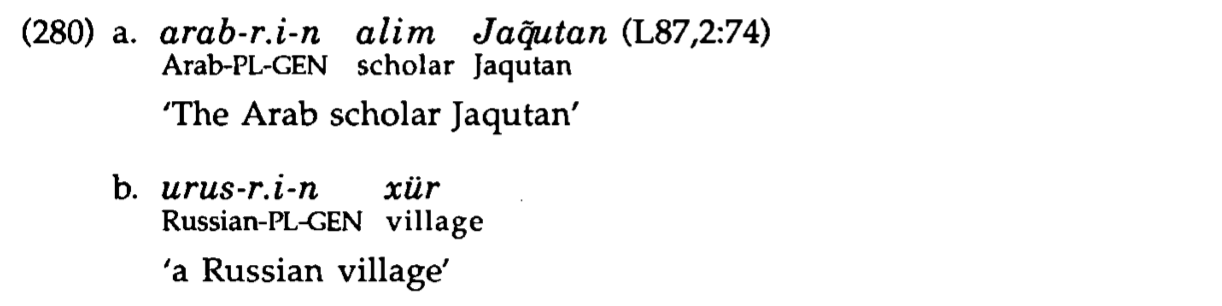
\includegraphics[width=.8\linewidth]{Lezgian/src/ex280.png}}
\end{figure}
\end{itemize}

\subsection{형용사의 파생}
\begin{itemize}
\item 동사에서 분사(동사형 형용사)를 파생시키는 다양한 접미사가 존재하고 9장에서 다룬다.
\end{itemize}

\subsubsection{파생 접미사}
\begin{itemize}
\item \textbf{-lu, -suz}
\begin{itemize}
\item \textbf{-lu} `having', \textbf{-suz} `suz'만이 자주 사용되는 생산적인 형용사화 접사이다.
\begin{figure}[H]
\centerline{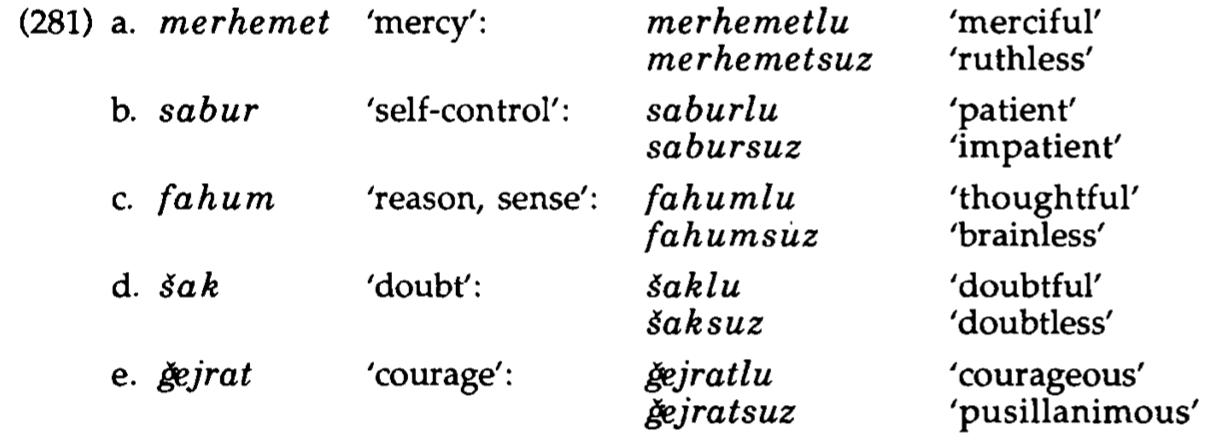
\includegraphics[width=.8\linewidth]{Lezgian/src/ex281.png}}
\end{figure}
\item 튀르크 차용어로, 주로 추상적 의미를 가진 동방 차용어에 부착된다.
\item 대부분의 경우 두 형태가 존재해서 반의어 쌍을 이루지만, 한 가지만 부착 가능한 경우도 있다.
\end{itemize}
\item \textbf{-U}
\begin{itemize}
\item 모음 조화에 따라 \textbf{-u/-ü/-i} 가 부착되는 접미사는 추상 명사로부터 형용사를 파생시키며 생산적이지는 않다.
\item 색깔이나 물리적 성질을 나타내는 아주 기본적인 단어들을 이루는 데에 사용된다.
\begin{figure}[H]
\centerline{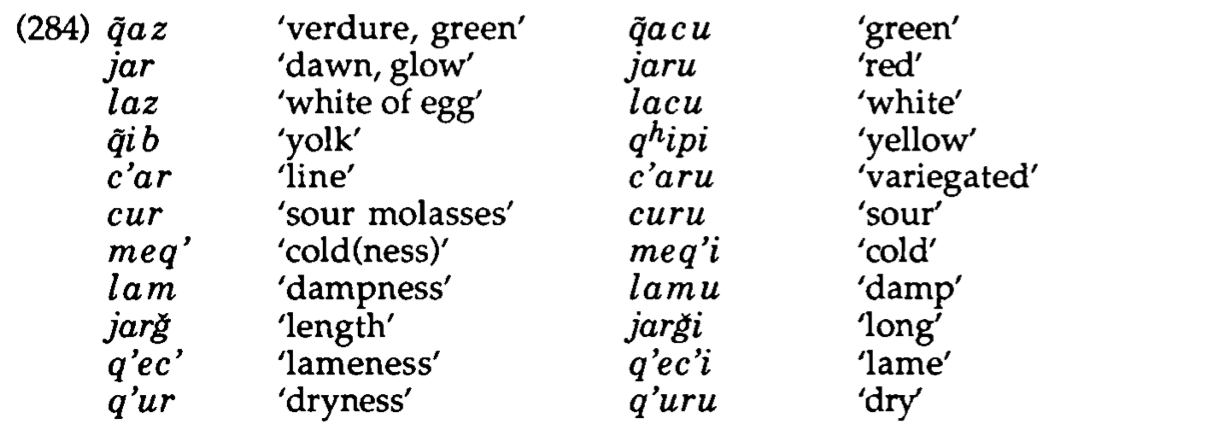
\includegraphics[width=.8\linewidth]{Lezgian/src/ex284.png}}
\end{figure}
\end{itemize}
\item \textbf{-an}
\begin{itemize}
\item \textbf{-an} 은 부사에서 형용사를 파생시킨다. 주로 시간 부사에 사용된다.
\begin{figure}[H]
\centerline{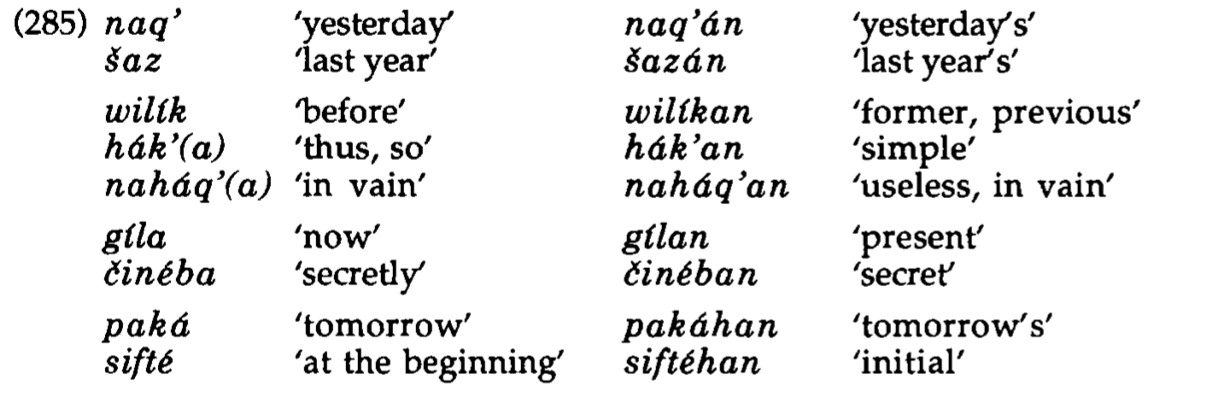
\includegraphics[width=.8\linewidth]{Lezgian/src/ex285.png}}
\end{figure}
\item 마지막 비강세 모음 뒤에서 \textbf{-n} 로 축약되고, 마지막 강세 모음 뒤에선 \textbf{h} 가 삽입된다. 
\item 속격 접미사 \textbf{-n} 와 형태적으로 유사하다.
\item 명사에서 파생되는 경우도 있다.
\begin{figure}[H]
\centerline{
\includegraphics[width=.8\linewidth]{Lezgian/src/ex286.png}}
\end{figure}
\item 몇몇 시간 부사는 같은 기능을 하는 접미사 \textbf{-nin} 를 취한다.
\begin{figure}[H]
\centerline{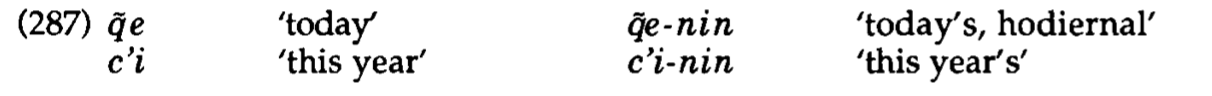
\includegraphics[width=.8\linewidth]{Lezgian/src/ex287.png}}
\end{figure}
\end{itemize}
\end{itemize}

\subsubsection{파생 접두사}
\begin{itemize}
\item \textbf{bej-}
\begin{itemize}
\item \textbf{bej-} `non, lacking-' 은 페르시아어 \textbf{bi-}에서 온 차용어이다. 
\begin{figure}[H]
\centerline{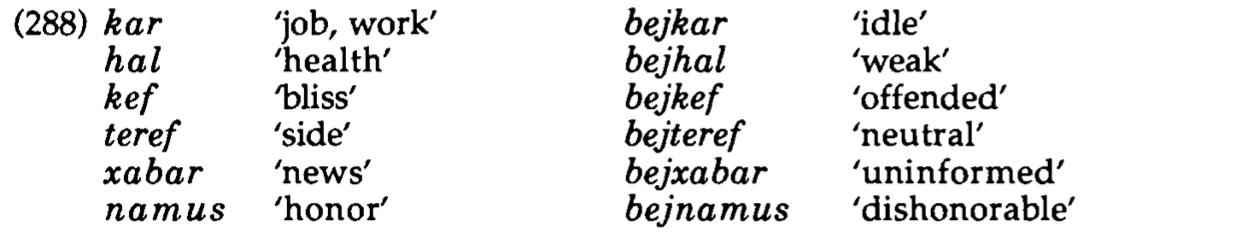
\includegraphics[width=.8\linewidth]{Lezgian/src/ex288.png}}
\end{figure}
\item 위 예시 중 몇몇은 시적 언어에만 제한적으로 사용된다.
\end{itemize}
\end{itemize}

%\section{동사 굴절}
%\subsection{서론}
%\subsection{강동사의 세 어간}
%\subsection{동사 굴절 범주}
%\subsection{부분적인 패러다임 예시}
%\subsection{불규칙 동사}
%\subsection{기본적인 시제-시상 범주의 기능}
%\subsection{완곡적 시제-시상 범주}
%\subsection{비-지시적 한정 동사 형태}
%\subsection{부정 동사 형태의 기능}
%\subsection{고어 형태}

















